\documentclass[main.tex]{subfiles}

\pagestyle{fancy}
%\fancyhf{}
\rhead{Assignment 3 - Re-Design of an Airfoil}
\lhead{AE4130 | 4738942}
\renewcommand{\headrulewidth}{0.1pt}
\begin{document}
\section{Problem Statement}
Modern airfoils can be designed using inverse methods and optimization techniques. In this assignment the task is to design an improved airfoil using the analysis and design program XFOIL. An aerodynamic analysis for a baseline airfoil, a NACA 4 series airfoil is performed and then reported. Clear plots of polars have been presented along with maximum $C_L/C_D$ values for mentioned boundary conditions. To improve the design of this baseline airfoil, the inverse airfoil design option in XFOIL has been exploited. The theory, procedure and reasoning behind each step has been discussed along with a comparative study for a NACA 6 series airfoil. An important note for this particular assignment is that for all the airfoils, the relative thickness($t/c$) is maintained.  
\section{Theory and Procedure}
In order to improve an airfoil, a study was performed to understand which characteristics of the airfoil are crucial in varying its lift/drag ratio. The baseline airfoil chosen for this study is the NACA 2212. The chosen airfoil has a maximum camber of 2\% and 20\% of the chord from the leading edge(see Table \ref{table1}). The result of having maximum camber so close to the leading edge(see Figure \ref{Fig1}) is that, suction pressure on the top surface of the airfoil increases. Also, like we saw in Assignment 2 the laminar separation can happen prematurely.\vspace*{-0.5em}
\\
\begin{table}[h]\begin{center}\begin{tabular}{ p{3cm} p{4.2cm} c } 
 \hline \rowcolor{lightgray}
  Digit & Meaning & Value\\
  \hline
 First Digit & Maximum Camber[\%] & 2 \\
 \hline
Second Digit & Max. Camber Pos.[\%] & 20  \\ 
\hline
Last 2 Digits & Max. Thickness[\%] & 12  \\ 
\hline
\end{tabular}\caption{NACA 4 digit name convention}\vspace*{-1em}\label{table1}\end{center}\end{table}\vspace*{-0.5em}
\\
The NACA 2212 is used as the baseline model to manually design an airfoil with improved laminar flow at the upper side of the wing, the procedure and results for this are discussed in later sections. The need to achieve an increased laminar flow is to avoid the flow to transition into a turbulent regime. Due to the nature of this airfoil profile, laminar transition happens early on. Although this might be considered beneficial , due to an increased lift, the studies in Figure \ref{fig3} show that it is only applicable for a small range of incidence angles($\alpha$). The Boundary conditions used for the analysis is shown in Table \ref{table2}.\vspace*{-0.5em}
\\
\begin{table}[h]\begin{center}\begin{tabular}{ c c } 
 \hline \rowcolor{lightgray}
  \hspace{0.5cm}Quantity\hspace{0.5cm} & \hspace{0.5cm}Value\hspace{0.5cm} \\
  \hline
  $\alpha$ & [-3:18]\\
 \hline
  R$_e$ & $1\times10^6$  \\ 
   \hline
  Mach & 0.0  \\ 
   \hline
  N$_{crit}$ & 9.0  \\ 
 \hline
  t/c$[\%]$ & 12.0  \\ 
\hline
\end{tabular}\caption{BCs used for this assignment}\vspace*{-1em}\label{table2}\end{center}\end{table}
\\
\begin{figure}[h!]
\vspace*{-4em}\centering
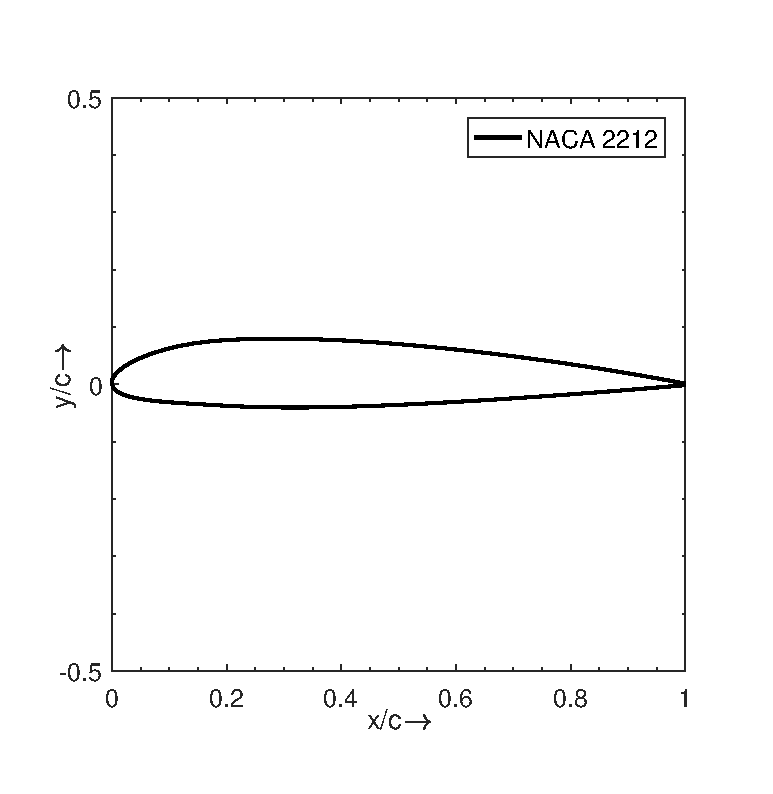
\includegraphics[width=0.45\textwidth]{./Images/Ass3/NACA2212}\vspace*{-1.3em}
\caption{NACA 2212 with max camber close to LE}\vspace*{-1.0em}
\label{Fig1}
\end{figure}\vspace*{-1.0em}
\\
\begin{figure}[h!]
    \vspace*{-2.5em}\centering
    \subfloat[Drag polar for NACA 2212]{
        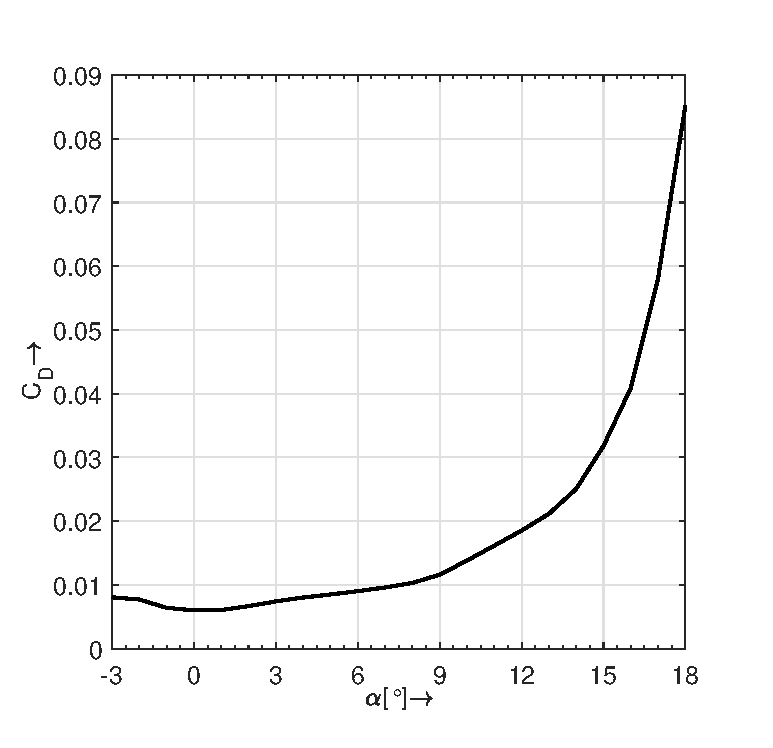
\includegraphics[width=0.45\textwidth] {./Images/Ass3/NACA2212Cdvsalpha}
        \label{fig2a} } \hspace*{-1.2em}
    \subfloat[Lift polar for NACA 2212]{
        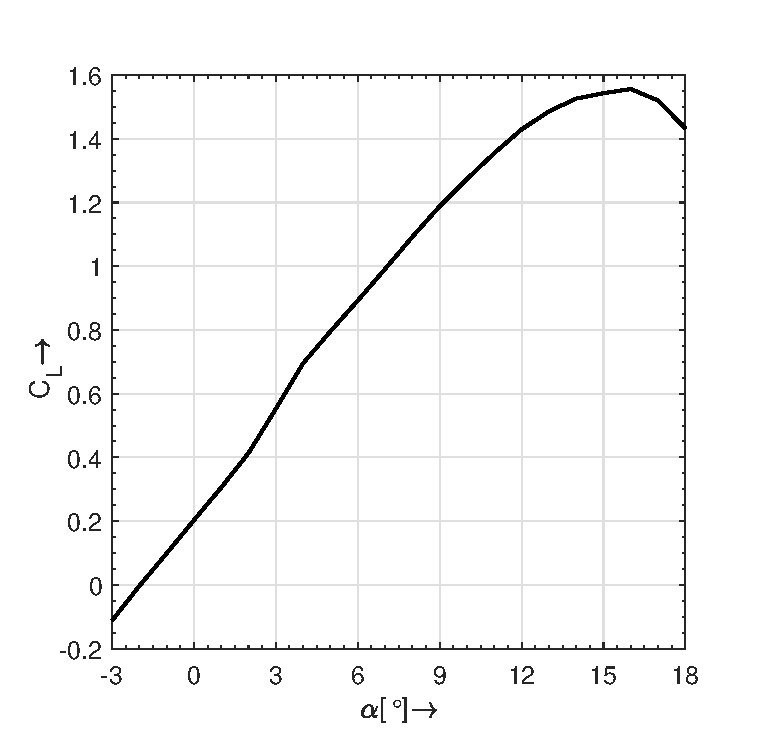
\includegraphics[width=0.45\textwidth] {./Images/Ass3/NACA2212Clvsalpha}
        \label{fig2b} } \\\vspace*{-1.0em}
         \subfloat[$C_L/C_D$ vs $\alpha$ for NACA 2212]{
        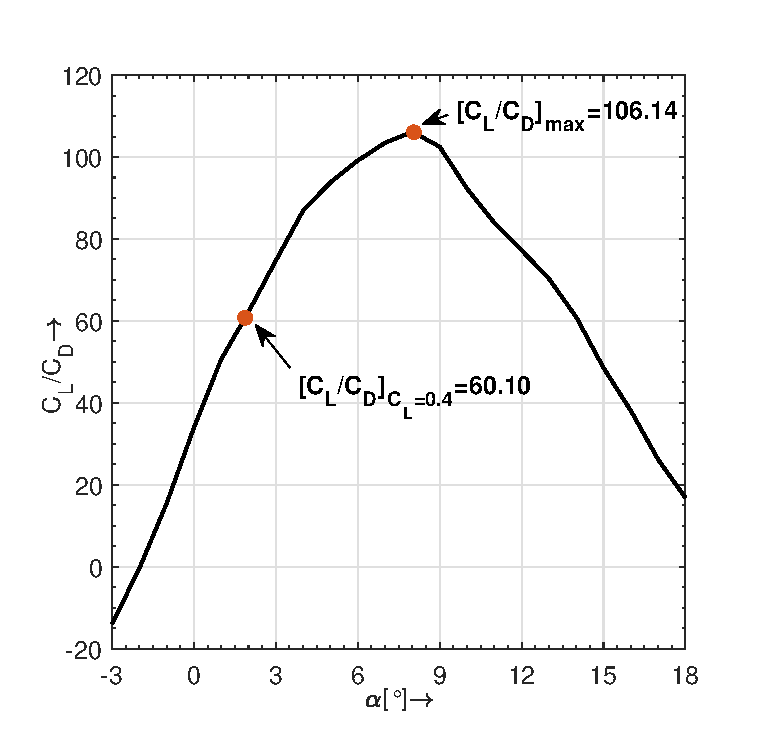
\includegraphics[width=0.45\textwidth] {./Images/Ass3/NACA2212ClCdvsalpha}
        \label{fig2c} } \hspace*{-1.2em}
    \subfloat[$C_P$ vs $x/c$ for NACA 2212]{
        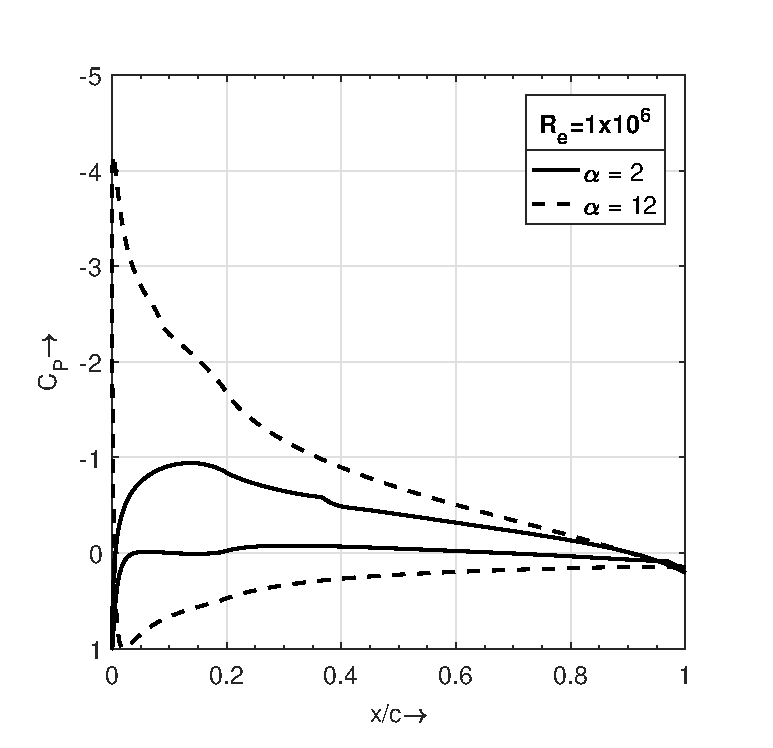
\includegraphics[width=0.45\textwidth] {./Images/Ass3/NACA2212_Cp}
        \label{fig2d} } \\\vspace*{-0.5em}
    \caption{Lift and Drag polar for NACA 2212}\vspace*{-1.9em}
    \label{fig2}
\end{figure}
\\\vspace*{-2.5em}
\par The first part of the assignment is to analyze the lift and drag characteristic for NACA 2212. Figure \ref{fig2} shows these results. The $C_P$ plot for $\alpha$=2 in Figure \ref{fig2d} shows a peak suction pressure, close to the LE. This is due to the presence of the max. thickness at 12$\%$ $t/c$. After this point, the pressure begins to drop. The maximum $C_L/C_D$ is 106.14 for an incidence angle of 8$^{\circ}$. When the C$_L$ value is set in XFOIL, we get a $C_L/C_D$ of 60.10. The airfoil starts to stall at about 16$^{\circ}$. This stalling behaviour is due to the increased pressure drag additional to the increased skin friction drag due to turbulence. The C$_m$ plot for this airfoil is shown in next section for comparison with the modified airfoil.
\subsection{Modification Procedure}
\par The purpose of modification is to improve the amount of laminar flow over the upper surface of the airfoil. For this, the software tool XFLR5 is used. XFLR5 is based on the same XFOIL code with a GUI. XFOIL allows us to modify the surface speed distribution of the entire airfoil geometry\cite{xfoilmanual}. Surface speed distribution($Q$) is linked to the pressure distribution($C_P$) over the airfoil, and hence is being exploited in a reverse engineering fashion. Since only the upper surface of the airfoil has to be modified, the mixed-inverse formulation method is used. The Mixed-Inverse formulation is simply the inviscid panel formulation (the discrete governing equations are identical) except that instead of the panel vortex strengths being the unknowns, the panel node coordinates are treated as unknowns wherever the surface speed is prescribed.  Only a part of the airfoil is altered at any one time\cite{xfoilmanual}.
\\
\par The \textit{XFOIL Inverse Design} option provides the user the capability to modify the surface speed distribution manually by drawing \textit{New Splines} over the existing curve. Since we are trying to modify only the upper wing surface, the \textit{Mark for Modification} tool is used to choose the start and end point of the wing surface. Since this is not an optimization tool, a number of iterations/modifications were tried out to understand how the surface speed affected the wing shape. Once an ideal surface speed curve is drawn, the \textit{Execute} command provides the new airfoil profile. But this changes the thickness, which is easily constrained using the \textit{Direct Foil Design} option under \textit{File Menu}. This modified airfoil is analyzed and has been reported in the next section. 
\\
\par Small changes in the airfoil profile caused large differences in convergence and polar plots. The steps which produced the best results are discussed below and the variations are shown in Figure \ref{fig3}:
\begin{itemize}
    \item The new surface speed distributions were always drawn higher than the original curve, so as to decrease the suction side pressure, thereby improving lift.
    \item The smoothness of the airfoil is very important for achieving XFOIL convergence. The splines near the LE and TE are carefully positioned so that negative thickness errors can be avoided.
    \item The spline is always drawn as a straight line in order to avoid adverse pressure gradients. Sometimes this caused convergence issues. A slight positive slope for the LE speed distribution fixed the issue.\\
\end{itemize}
\pagebreak
\begin{figure}[t]
\centering
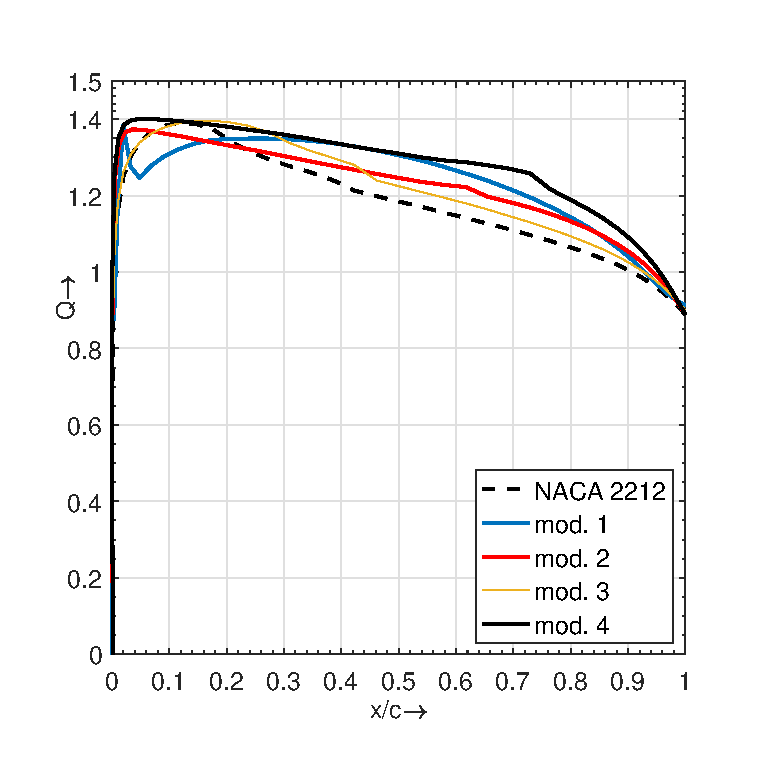
\includegraphics[width=0.5\textwidth]{./Images/Ass3/QvsX_mod}
\caption{Variations of surface speed distributions}
\label{fig3}
\end{figure}

\section{Results and Discussions}
\subsection{NACA 2212 vs Modified Airfoils}
\begin{figure}[h]
\vspace*{-1em}
\centering
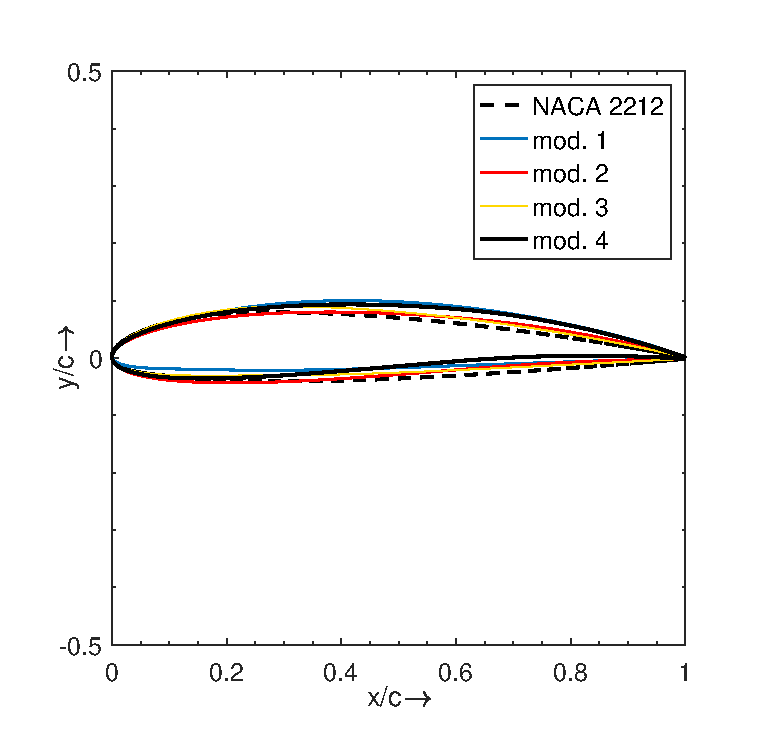
\includegraphics[width=0.5\textwidth]{./Images/Ass3/Airfoil_Comp}
\caption{Comparison of modified airfoils}
\label{fig4}
\vspace*{-1em}
\end{figure}
\\ The various airfoil modifications($mod.$) obtained through the study are shown in Figure \ref{fig4}. While trying to improve the laminar flow, it is observed that the location of maximum thickness keeps shifting downstream slightly(all the while it is still maintained at t/c=12\%). This corroborates the facts stated about laminar transition in Assignment 2. The modified airfoils also have a maximum change of 50\% in the camber. This happens to account for the shift in max thickness location. The lift and drag characteristics for these various modifications are shown in Figure \ref{fig5}
\begin{figure}[h!]
    \vspace*{-1.5em}\centering
    \subfloat[C$_L$ vs $\alpha$]{
        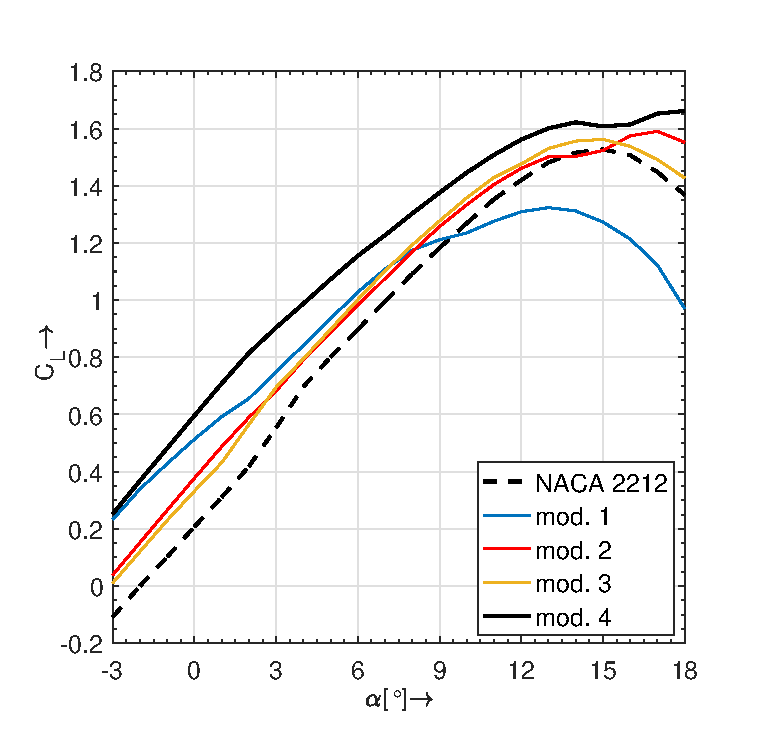
\includegraphics[width=0.5\textwidth] {./Images/Ass3/Cl_comp}
        \label{fig5a} } \hspace*{-1.2em}
    \subfloat[$C_L$ vs $C_D$]{
        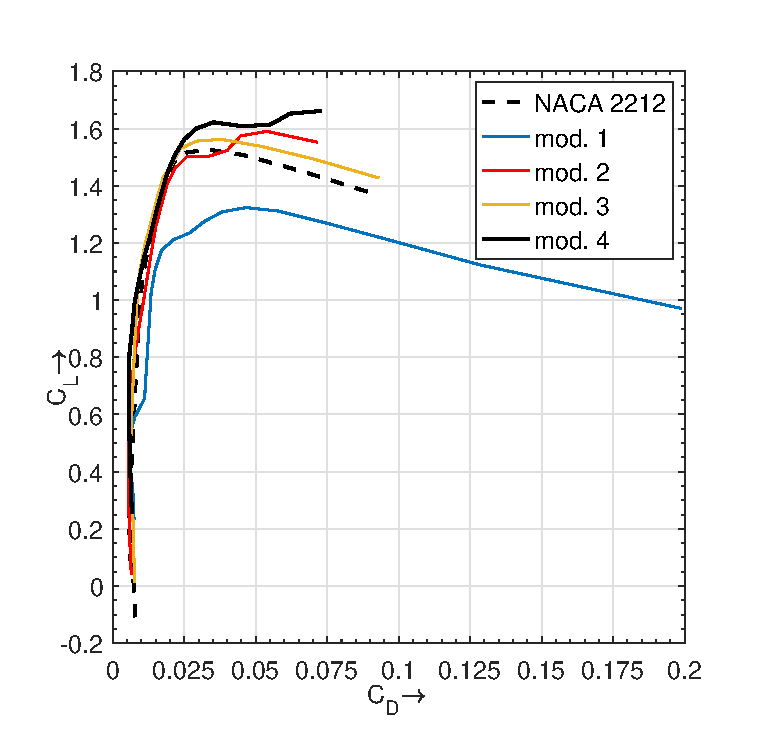
\includegraphics[width=0.5\textwidth] {./Images/Ass3/ClvsCd_comp}
        \label{fig5b} } \\\vspace*{-1.1em}
         \subfloat[$C_L/C_D$ vs $\alpha$]{
        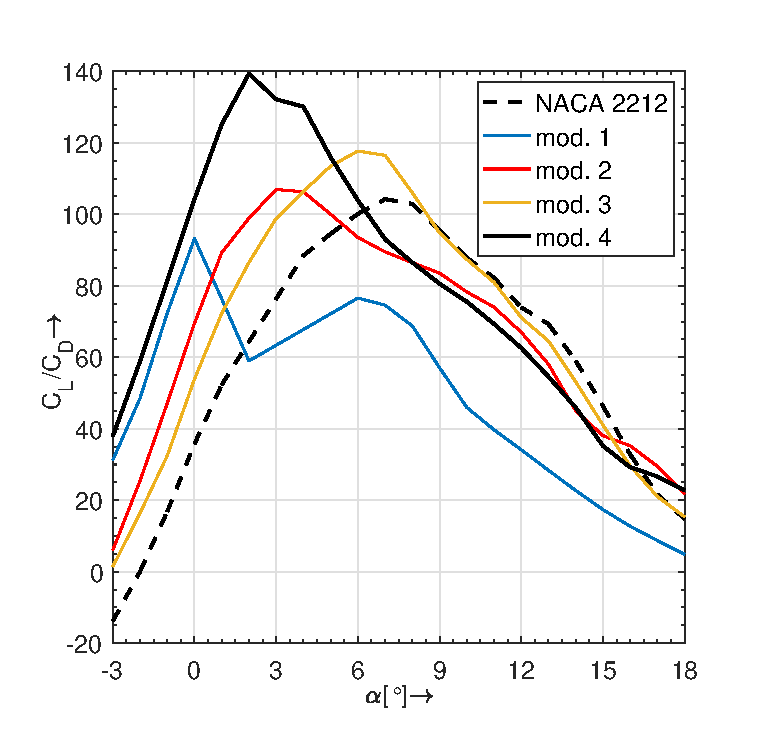
\includegraphics[width=0.5\textwidth] {./Images/Ass3/ClCdvsAlpha_comp}
        \label{fig5c} } \hspace*{-1.2em}
    \subfloat[$C_m$ vs $\alpha$]{
        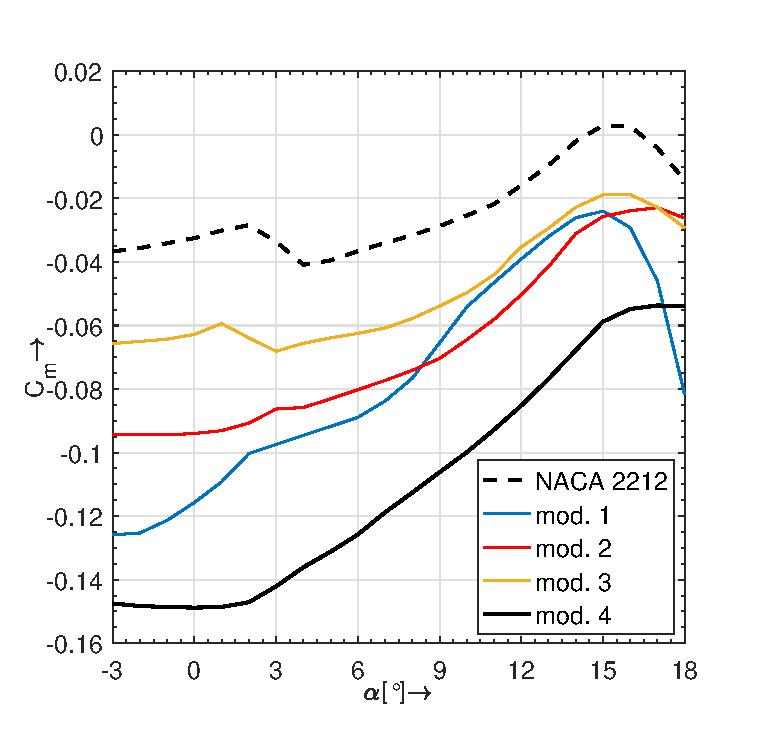
\includegraphics[width=0.5\textwidth] {./Images/Ass3/CmvsAlpha_comp}
        \label{fig5d} } \\
    \caption{Lift and Drag polar for various modifications}
    \label{fig5}
\end{figure}\\
\par\vspace*{-1.5em} Analyzing Figure \ref{fig5a}, its evident that shifting the speed distribution above the original curve has improved the lift characteristics. This effect is conspicuous at lower angle of attacks, mostly because of the smoothness of the new splines in Figure \ref{fig3}. The first modification shows poor stalling characteristics due to improper blending of the leading edge spline with the original curve. This is corrected in further modifications and shown as \textit{mod. 2, mod. 3} and \textit{mod. 4} respectively. The 4$^{th}$ modification gave the best result due to the improved lift performance even at higher incidence angles. This is possibly because \textit{mod. 4} has the maximum camber at about 61.7\% from LE. \textit{mod. 4} also has the best lift to drag ratio in Figure \ref{fig5c} for lower incidence angles. When compared to NACA 2212, a 32\% increase in maximum lift to drag is observed. This is due to the improved length of laminar region over the upper surface. For $\alpha$ more than 6$^\circ$, the adverse pressure gradient becomes more prominent. The skin friction drag due to the inevitable laminar separation bubble also starts to contribute to the total drag.
\\\par The comparison of pitching moment($C_m$) is shown in Figure \ref{fig5d}. The $C_m$ vs $\alpha$ plot is very useful in identifying whether an airfoil is stable at higher incidence angles. NACA 2212 shows a slightly positive $C_m$ at its stalling angle. This means that this airfoil will pitch clockwise when it stalls, whereas the modified airfoils especially \textit{mod. 4} has a counter-clockwise pitching moment throughout the incidence regime. This denotes an improvement in the stalling performance for the modified airfoils.
\subsection{Optimized Airfoil vs NACA 64012A}
\begin{figure}[h]
\vspace*{-1em}
\centering
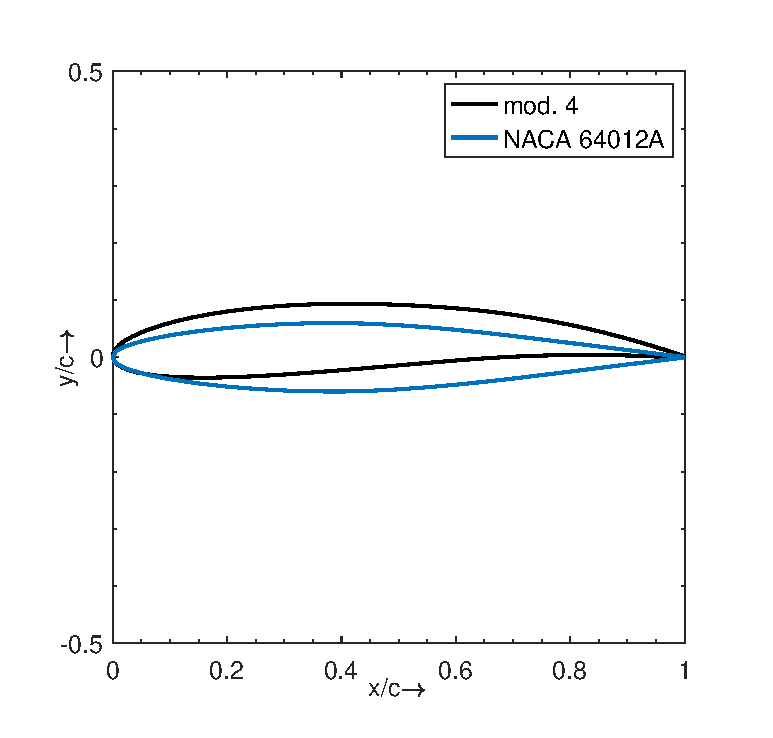
\includegraphics[width=0.5\textwidth]{./Images/Ass3/Final_Airfoil_Comp}
\caption{Comparison of modified airfoil with NACA 64012A}
\label{fig6}
\vspace*{-1em}
\end{figure}
\par With the same approach as above, a comparative study between \textit{mod. 4} and NACA 64012A\cite{airfoiltools} has been made. The profiles comparison and the polar plots are presented in Figure \ref{fig6} and \ref{fig7} respectively. Its is very evident from the results that the modified airfoil performs better than NACA 64012A for all incidence angles. NACA 64012A starts to stall at 12$^\circ$ due to the early laminar separation of the boundary layer. This shows that modification procedure followed has worked well in achieving an extended laminar region. The continuously increasing C$_D$ even after the stall at C$_D=0.031$(see Figure \ref{fig7d}) is due to the adverse pressure gradient(pressure drag) that keeps worsening with increasing $\alpha$. Manually adjusting the speed distribution with the help of XFOIl inverse airfoil has been elemental in decreasing the adverse pressure gradient towards the rear end of the airfoil. The pitching moment behaviour is particularly bad for the NACA 64012A. The wing would destabilize even at lower incidence angles. As mentioned before, pitching moment for \textit{mod. 4}, although increases, it is not as destabilizing as for NACA 64012A. This is because the chosen NACA airfoil has very less camber, which was the case for NACA 2212 as well. 
\begin{figure}[h!]
    \vspace*{-1.5em}\centering
    \subfloat[C$_L$ vs $\alpha$]{
        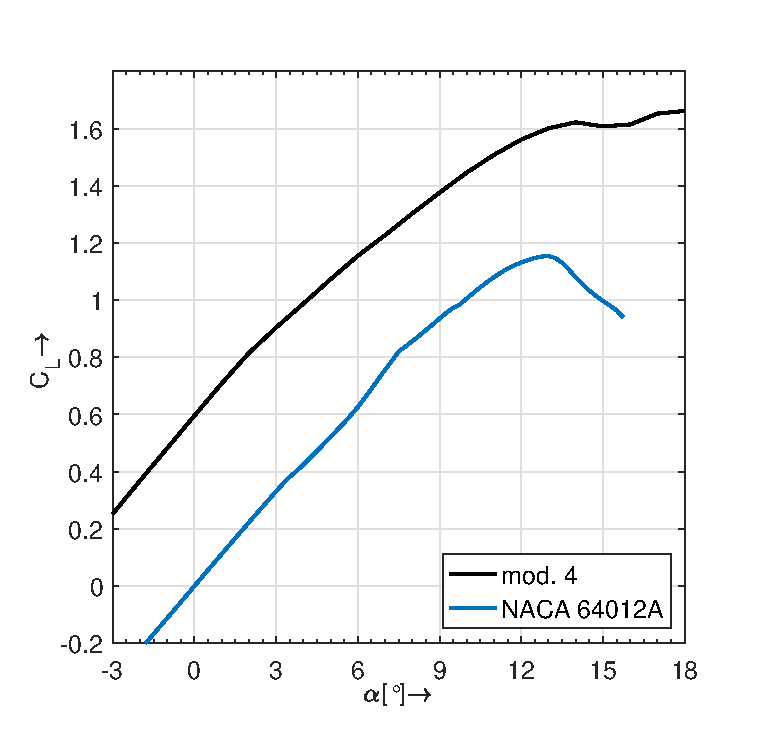
\includegraphics[width=0.5\textwidth] {./Images/Ass3/Final_Cl_comp}
        \label{fig7a} } \hspace*{-1.2em}
    \subfloat[$C_L$ vs $C_D$]{
        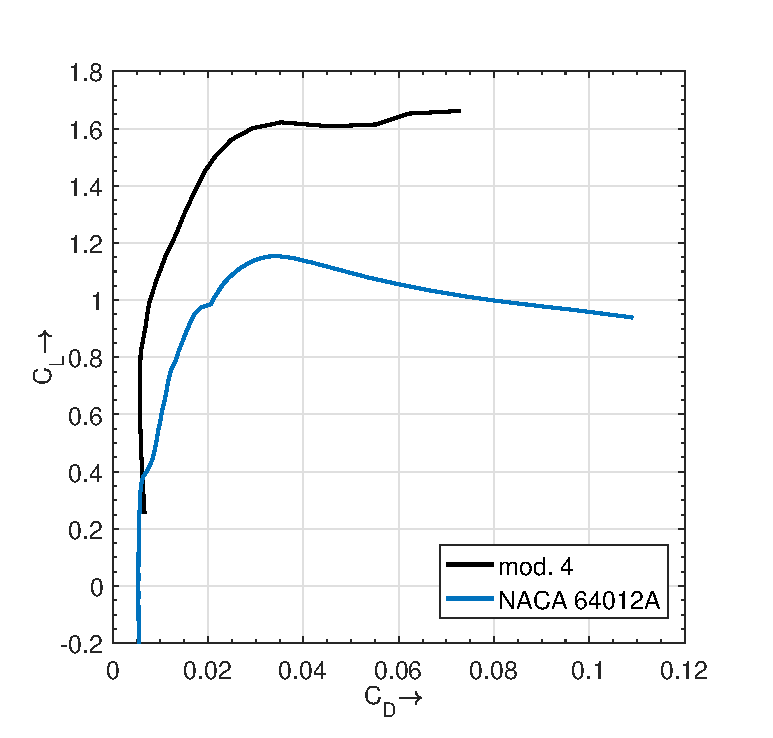
\includegraphics[width=0.5\textwidth] {./Images/Ass3/Final_ClvsCd_comp}
        \label{fig7b} } \\\vspace*{-1.1em}
         \subfloat[$C_L/C_D$ vs $\alpha$]{
        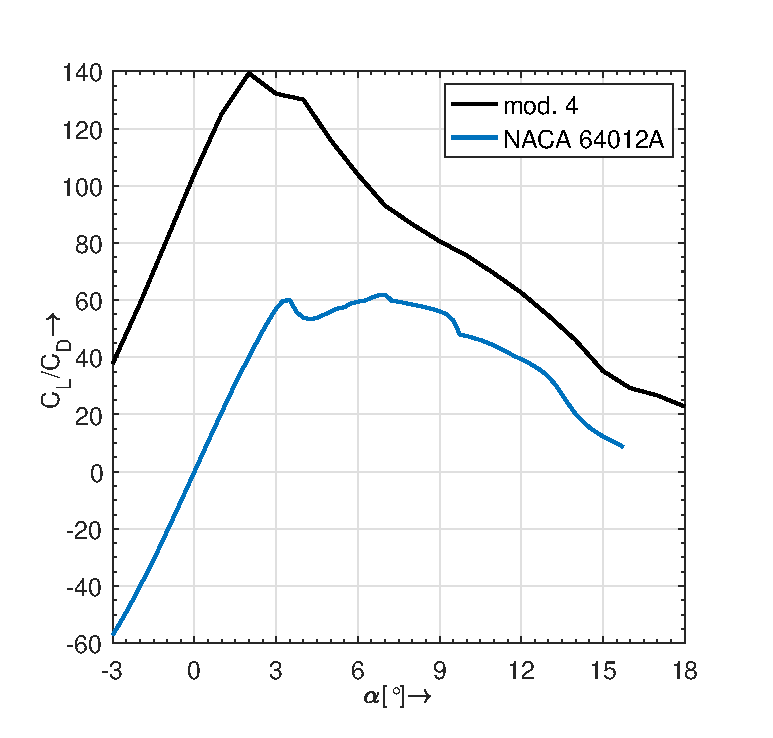
\includegraphics[width=0.5\textwidth] {./Images/Ass3/Final_ClCdvsAlpha_comp}
        \label{fig7c} } \hspace*{-1.2em}
    \subfloat[$C_m$ vs $\alpha$]{
        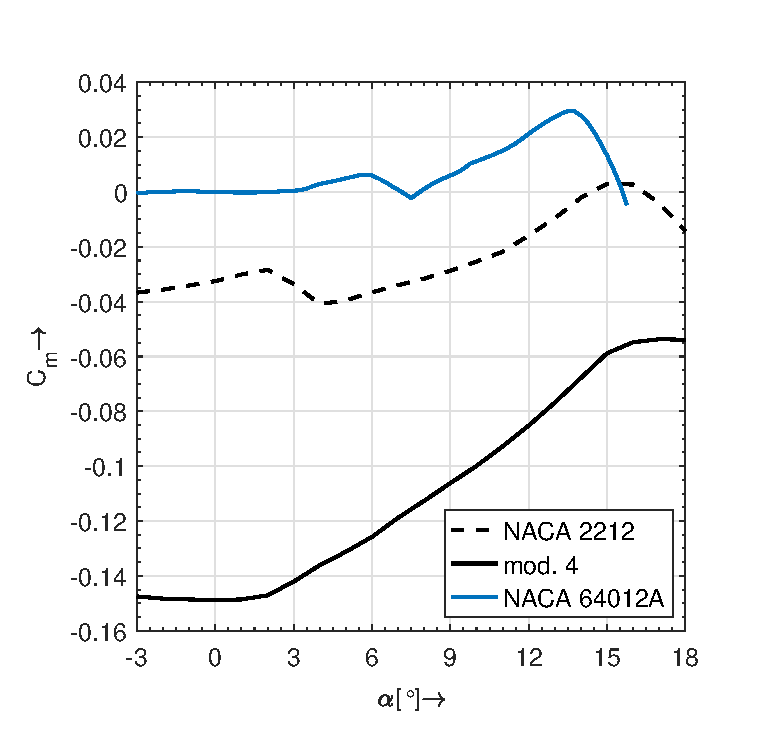
\includegraphics[width=0.5\textwidth] {./Images/Ass3/Final_CmvsAlpha_comp}
        \label{fig7d} } \\
    \caption{Lift and Drag polar for $mod. 4$ and NACA 64012A}\vspace*{-1.5em}
    \label{fig7}
\end{figure}\\
\\\par From these studies it is evident that the modified airfoil labelled as \textit{mod. 4} is definitely an improved profile with better lift to drag performance characteristic. Satisfactory reasoning for the design measures taken in producing such an optimized airfoil profile has also been presented. It has also been pointed out how increasing the laminar flow regime has affected/improved the flow over the wing.

\printbibliography[title={References}]
\end{document}
